\appendices

\section{Periodic neural SDE toy study}
\label{app:periodic-toy-study}

This preliminary study illustrates coefficient learning for the periodic SDE
in Equation~\eqref{eq:periodic-toy-sde}, with true drift $b(x)=-\sin x$,
constant diffusion amplitude $\sigma=1.1$, and initial state $X_0=0$.
It explores observation spacing, trajectory duration, and fitting choices;
it is not evidence answering the equity-return research question.
The observation-spacing comparison is shown in Figure~\ref{fig:repeated-density}
in Section~\ref{sec:observation-spacing-example}.

\subsection{Network structure}

For the periodic-potential experiment, the drift network receives
$(\sin x,\cos x)$ as inputs. This enforces the known period $2\pi$, appropriate
to the generating drift $b(x)=-\sin x$. Its four hidden layers each contain 64 units
with hyperbolic-tangent activation. The architecture learns the shape of the
periodic drift while incorporating prior knowledge of its period.

The active diffusion model is a single learned positive scalar, using the
softplus function \parencite{Goodfellow2016}:
\begin{equation}
    s_\theta(x)=\operatorname{softplus}(\rho)+\varepsilon,
    \qquad \operatorname{softplus}(\rho)=\log(1+e^\rho),
    \qquad \varepsilon=10^{-3}.
    \label{eq:positive-diffusion}
\end{equation}
Thus the experiments learn a neural drift and constant diffusion. Positivity
avoids the sign ambiguity of a scalar diffusion amplitude when identifying its
law through $s_\theta^2$.

\subsection{Simulation and training settings}

The comparisons below use 50 training trajectories, simulated over $T=500$
with 15,000 saved observations per path. The saved spacing is approximately
$0.03334$, with four Euler integration steps per observation interval.
Subsampling or truncating these paths changes the observation spacing or
duration while preserving the underlying numerical simulation.

Each configuration is fitted five times with new training data and training
seeds. Configurations within a repeat share the training pool and seed.
Training uses Adam with learning rate $10^{-3}$, minibatches of 2,048
increments, and 1,500 updates. Checkpoints are selected using a fixed sample
of 4,096 held-out increments at the original fine observation spacing,
including the untrained model as a candidate. Coefficient errors follow
Equation~\eqref{eq:coefficient-errors}, with drift evaluated on 512 uniformly
spaced points over one period. The figures report medians and interquartile
ranges across five fits; the bands describe variation between runs, rather
than confidence intervals.

The implementation averages the first two terms in
Equation~\eqref{eq:neural-sde-nll}, omitting the final term because it does
not depend on the learned parameters. Actual elapsed times $h_i$ enter the
loss, including when selecting a subset of saved observations.
Adam \parencite{KingmaBa2015} performs parameter updates using randomly
sampled minibatches.

\subsection{Evaluation}

Because the data are simulated, we know the true drift and diffusion. We can
therefore compare them directly with the learned values. To check the drift,
we evaluate both functions at the same $Q$ evenly spaced positions $x_q$
covering one period. The percentage errors are
\begin{equation}
    E_b=100\sqrt{
       \frac{\sum_{q=1}^{Q}[b_\theta(x_q)-b(x_q)]^2}
            {\sum_{q=1}^{Q}b(x_q)^2}},\qquad
    E_\sigma=100\frac{|\widehat{\sigma}-\sigma|}{\sigma}.
    \label{eq:coefficient-errors}
\end{equation}
Here $b$ is the true drift, $b_\theta$ is the learned drift, $\sigma$ is the
true diffusion amplitude, and $\widehat{\sigma}$ is its learned value.
The drift error $E_b$ combines the differences across the sampled positions
and expresses their size relative to the true drift. The diffusion error
$E_\sigma$ is the difference between the learned and true amplitudes,
relative to the true amplitude. Zero means an exact match at the evaluated
positions for drift, or an exact match of the amplitude for diffusion.
These relative errors require at least one nonzero true drift value on the
evaluation grid and $\sigma>0$.

We also check the loss on observations not used for training and compare
the final positions of simulated trajectories. These checks answer different
questions: the loss measures how well the model explains observed increments,
while the final positions show its behavior over a longer time. A low
validation loss or similar final-position distributions do not by themselves
guarantee that the learned drift and diffusion are correct. In particular,
at short observation intervals, drift errors can have little effect on the
loss because their contribution is small relative to the noise.

The amount of data also needs to be described carefully. With $M$ trajectories
and $K$ observations per trajectory, there are $M(K-1)$ observed increments.
However, the same increment count can come from densely sampled short paths
or sparsely sampled long paths. These need not be equally useful for learning
the coefficients, so the experiments distinguish observation spacing,
trajectory duration, and the number of independent trajectories.

\subsection{Findings}

\paragraph{Observation spacing and diffusion recovery.}

At fixed duration $T=500$, increasing the number of observations per path
reduces the distance in time between observations.
Figure~\ref{fig:repeated-density} in Theory shows that median diffusion error
decreases from $18.18\%$ at spacing $\Delta t\approx1.00$ to $0.86\%$ at
$\Delta t\approx0.03334$. Drift error initially improves as the coarsest
sampling is refined, but does not continue to decrease with denser sampling:
its median is $8.45\%$ at 3,000 observations and $10.72\%$ at 15,000.
Thus, once the coarsest intervals are excluded, finer sampling benefits
diffusion recovery more consistently than drift recovery in this example.

This distinction is consistent with the local increment model in
Equation~\eqref{eq:local-gaussian}: the drift contribution scales with
$\Delta t$, while the random contribution scales with $\sqrt{\Delta t}$.
Reducing the interval therefore makes the drift contribution smaller relative
to the noise in each increment. More frequent observations over the same time
span need not improve drift recovery in the same way as diffusion recovery.

\paragraph{Trajectory duration and drift recovery.}

The duration comparison keeps observation spacing approximately $0.03334$
and uses progressively longer prefixes of the same paths.
In Figure~\ref{fig:repeated-duration}, median drift error decreases overall
from $17.08\%$ at $T\approx33.30$ to $10.72\%$ at $T=500$, although the
intermediate values fluctuate. Diffusion error is already small at the
shortest duration: its median changes from $1.11\%$ to $0.86\%$ between
these endpoints.

\begin{figure}[htbp]
    \centering
    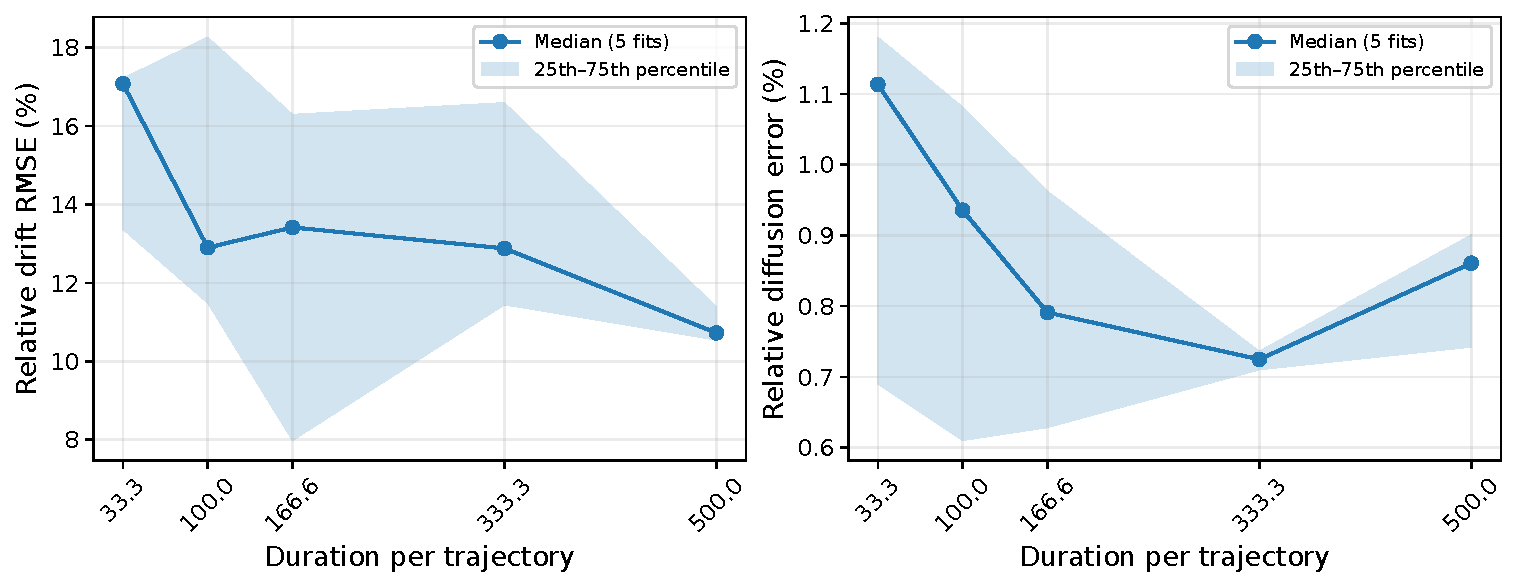
\includegraphics[width=0.9\linewidth]{figures/results/repeated-duration.pdf}
    \caption{Exploratory duration sweep with 50 training trajectories and
    fixed observation spacing $\Delta t\approx0.03334$. Lines show median
    coefficient errors over five fits; bands show the 25th--75th percentiles.}
    \label{fig:repeated-duration}
\end{figure}

The comparison illustrates why observation spacing and total observation time
should be distinguished. Longer trajectories provide additional time over
which to observe the systematic drift, whereas denser sampling resolves
short-time fluctuations. Here, extending duration gives an overall improvement
in drift recovery that is absent when only the already fine sampling is made
denser. This is an observed tendency, not a monotonic learning curve or a
separation of the two coefficients: both depend on the data and fitting
procedure.

\paragraph{Coarse sampling and validation at the original scale.}

The coarsest configuration exposes a limitation of the fitting approach.
With 500 observations over $T=500$, training intervals are approximately
$1.00$, while validation intervals remain approximately $0.03334$.
Four of the five fits select the untrained initial checkpoint: none of their
evaluated trained checkpoints improves its fine-scale validation loss.
The selected diffusion remains at its initial value $0.9$, giving
$18.18\%$ error relative to the true amplitude $1.1$. Two extended checks
still select the untrained checkpoint after 6,000 updates. In this specific
validation sense, the untrained model performs better than the evaluated
trained models, despite having inaccurate coefficients itself.

A plausible explanation is the mismatch between a local Gaussian transition
model and increments spanning a long interval. The loss approximates the drift
and diffusion as constant within each interval. Over a coarse interval, the
state can move through regions with different drift, so the observed
displacement combines dynamics that this approximation does not resolve.
Fitting it can therefore favor coefficients that represent finite-interval
transitions rather than the original instantaneous SDE coefficients. Such a
representation need not transfer to the original fine time scale used for
validation. Coarse sampling leaves the generating SDE unchanged, but obscures
the within-interval dynamics in the observations used by this loss.

The checkpoint results demonstrate the failure to improve fine-scale
validation in these runs. They are consistent with this approximation-error
explanation, but do not isolate it from optimization effects or establish that
the trained models accurately fit the coarse transitions. The practical lesson
of these exploratory examples is that observation spacing, trajectory duration,
and the time scale assumed by the loss all matter when interpreting learned
SDE coefficients. Full experiment details and outputs remain in
\texttt{likelihood\_calc.ipynb}, \texttt{sde\_test\_data.ipynb}, and
\texttt{sandbox/experiments/experiment\_results}.
